% !TEX root = main.tex

\section{凸优化问题}
\subsection{标准型}
\label{sub:convex_opt_def}
广义定义:极小化凸函数,约束为凸集
\[\begin{aligned}
& \text{minimize}& f_0(\vx)& &\\
& \text{subject to}& f_i(\vx)&\leq 0 &\quad i&=1,\ldots,m\\
&  & h_j(\vx)&=0 &\quad j&=1,\ldots,p
\end{aligned}\]
\begin{itemize}
	\item 优化变量$\vx\in\rn$
	\item 目标/损失函数$f_0:\rn\mapsto \rr$
	\item 不等式约束函数$f_i:\rn\mapsto \rr$
	\item 等式约束函数$h_j:\rn\mapsto\rr$
	\item 域$\sD=\bigcap_{i=0}^m\dom f_i\cap\bigcap_{i=1}^p\dom h_i$
	\item 可行解$\sX=\{\vz\mid f_i(\vz)\leq 0,h_j(\vz)=0,i=1,\ldots,m,j=1,\ldots,p\}$
	\item 最优值$P^\star=\inf\{f_0(\vx)\mid \vx\in \sX\}$
	\item 最优解$\vx^\star\iff\forall \vz\in\rn,\vz\in\sX:\;f_0(\vz)\geq f_0(\vx^\star)$
	\item 最优解集$X^\star=\{\vx^\star\mid f_0(\vx^\star)=P^\star,\vx^\star\in \sS\}$
	\item $\eps$-次优解集$X_\eps=\{\vx\mid f_0(\vx)\leq P^\star+\eps, \vx\in \sX\}$
	\item 局部最优$\exists R>0,f_0(\vx)=\inf\{f_0(\vz)\mid \vx\in\sX, \vz\in\sX,\|\vx-\vz\|\leq R\}$,即邻域内下确界
	\item 局部最优解集$x_{local}=\{\vx\mid\vx\text{为局部最优}\}$
\end{itemize}

狭义定义:$f_i(\vx),i=0,1,\ldots$为凸函数,$h_i(\vx)$为仿射函数
\begin{example}
\begin{mini*}
	{}{f_0(x)=x_1^2+x_2^2}{}{}
	\addConstraint{f_1(x)}{=\frac{x_1}{1+x_2^2}\leq 0}{\implies x_1\leq 0}
	\addConstraint{h_1(x)}{=(x_1+x_2)^2=0}{\implies x_1+x_2=0}
\end{mini*}
\end{example}

% 3.19
\begin{theorem}
凸问题局部最优等价于全局最优
\end{theorem}
\begin{analysis}
若$\vx$为局部最优
\[\exists R>0:\;f_0(\vx)=\inf\{f_0(\vz)\mid \vz\in\sX,\vx\in\sX,\|\vx-\vz\|_2\leq R\}\]
反证法,设$\vx$不是全局最优,$\vy$为全局最优,即$f_0(\vx)>f_0(\vy)$\\
取$\vz=\theta \vx+(1-\theta)\vy$为$\vx,\vy$连线上一点,令$\theta=\frac{R}{2\|\vy-\vx\|_2}$,使$\vz$能够落在$\vx$的邻域内
\[\|\vz-\vx\|_2=\frac{R\|\vy-\vx\|_2}{2\|\vy-\vx\|_2}=\frac{R}{2}\]
由$\|\vz-\vx\|_2\leq R\implies f_0(\vx)\leq f_0(\vz)$,又结合$f_0(\vx)>f_0(\vy)$,有
\[f_0(\vz)\leq\theta f_0(\vx)+(1-\theta)f_0(\vy)<\theta f_0(\vz)+(1-\theta)f_0(\vz)=f_0(\vz)\]
左边第一个不等号由凸函数定义,第二个不等号由推导出的条件,故矛盾
\end{analysis}

对于可微凸目标函数$f_0(\vx)$,最优解满足以下条件
\begin{itemize}
	\item 无约束$\min f_0(\vx)$,只需$\nabla f_0(\vx^\star)=0$
	\begin{analysis}
	由凸函数的性质
	\[\forall \vx,\vy:\;f_0(\vy)\geq f_0(\vx)+\lrang{\nabla f_0(\vx),\vy-\vx}\]
	进而
	\[f_0(\vy)\geq f_0(\vx^\star)+\lrang{\nabla f_0(\vx^\star),\vy-\vx}=f_0(\vx^\star)\]
	\end{analysis}
	\item 有约束$\min f_0(\vx),\,s.t.\,\vx\in\sX$
	\[\forall \vy\in \sX:\lrang{\nabla f_0(\vx^\star),\vy-\vx^\star}\geq 0\]
	\begin{figure}[H]
		\centering
		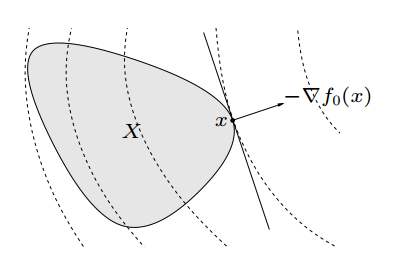
\includegraphics[width=0.4\linewidth]{fig/optimal_criterion_diff.PNG}
	\end{figure}
\end{itemize}

\begin{example}
等式约束 $\min f_0(\vx),\dom f_0\subset\rn$,$f_0$可微,使得$A\vx=\vb$
\end{example}
\begin{analysis}
$\vx^\star$最优,$A\vx^\star=\vb$,最优解需满足
\[\forall \vy, A\vy=\vb:\;\lrang{\nabla f_0(\vx^\star),\vy-\vx^\star}\geq 0\]
从而
\[\begin{cases} \vy=\vx^\star+\vv\\A\vv=\vzero\end{cases},\vv\in\opnul A\]
即
\[\forall \vv\in\opnul A:\;\lrang{\nabla f_0(\vx^\star),\vv}\geq 0\]
那么
\begin{enumerate}
	\item $\opnul A=\{\vzero\}$
	\item $A$不可逆,$\nabla f_0(\vx^\star)\perp\opnul A$
\end{enumerate}
\end{analysis}

\begin{example}
正约束$\min f_0(\vx),s.t.\,\vx\geq\vzero$
\end{example}
\begin{analysis}
若$\vx^\star$最优$\iff \vx^\star\geq \vzero,\forall \vy\geq \vzero,\lrang{\nabla f_0(\vx^\star),\vy-\vx^\star}\geq 0
\iff \lrang{\nabla f_0(\vx^\star),\vy}\geq\lrang{\nabla f_0(\vx^\star),\vx^\star}$
\begin{enumerate}
\item 若$\nabla f_0(\vx^\star)\ngeq 0$,则存在矛盾(负数行乘上正无穷),故$\nabla f_0(\vx^\star)\geq 0$
\item 令$\vy=0$,有$0\geq \lrang{\nabla f_0(\vx^\star),\vx^\star}
\implies\sum_{i=1}^n(\nabla f_0(\vx^\star))_ix_i^\star\leq 0$\\
前面$\geq 0$,进而互补松弛条件
\item $\vx^\star\geq 0$
\end{enumerate}
\end{analysis}

\subsection{线性规划}
\begin{mini*}
	{}{\vc^\T\vx+\vd}{}{}
	\addConstraint{G\vx}{\leq\vh}
	\addConstraint{A\vx}{=\vb}
\end{mini*}

\begin{example}[食谱问题]
$m$种营养元素不小于$b_1,\ldots,b_m$,$n$种食物,单位含量$a_{1j},\ldots,a_{mj}$,食物量$x_1,\ldots,x_n$,价格$c_1,\ldots,c_n$
\begin{mini*}
	{}{\sum_{i=1}^n c_jx_j}{}{}
	\addConstraint{\sum_{j=1}^n a_{ij}x_j}{\geq b_i}
	\addConstraint{x_j}{\geq 0}
\end{mini*}
其中$i=1,\ldots,m,j=1,\ldots,n$
\end{example}

% 3.21
\begin{example}[线性分数规划]
\begin{mini*}
	{}{f_0(\vx)=\frac{\vc^\T \vx+d}{\ve^\T \vx+f}, \dom \vf=\{\vx \mid \ve^\T \vx + f >0 \}}{}{}
	\addConstraint{G\vx}{\leq \vh}
	\addConstraint{A\vx}{=\vb}
\end{mini*}
等价于
\begin{mini*}
	{}{\vc^\T \vy+dz}{}{}
	\addConstraint{G\vy-hz}{\leq 0}
	\addConstraint{A\vy-bz}{=0}
	\addConstraint{\ve^\T \vy+fz}{=1}
	\addConstraint{z}{\geq 0}
\end{mini*}
\end{example}
\begin{analysis}
	证明两个问题等价,$P_0$与$P_1$\\
	若$\vx$在$P_0$内可行
	\[\vy=\frac{\vx}{\ve^\T \vx+f},z=\frac{1}{\ve^\T \vx+f}\]
	若$(\vy,z)$在$P_1$中可行
	\[\vx=\frac{\vy}{z}(z\ne 0)\]
	若$z=0$,$x_0$为$P_0$的可行解
	\[\vx=\vx_0+t\vy,t\geq 0\]
	\[\lim_{t\to\infty}\frac{\vc^\T(\vx_0+t\vy)+d}{\ve^\T(\vx_0+t\vy)+f}=\vc^\T \vy\]%考试
	代入看所有条件结论都相同
\end{analysis}

\subsection{二次规划}
二次规划(Quadratic Programming)
\begin{mini*}
	{}{\frac{1}{2}\vx^\T P\vx+\vq^\T\vx+r,\;P\succ 0}{}{}
	\addConstraint{G\vx}{\leq h}
	\addConstraint{A\vx}{=\vb}
\end{mini*}

二次约束二次规划(QCQP)
\begin{mini*}
	{}{\frac{1}{2}\vx^\T P_0\vx+\vq_0^\T \vx+r_0,P_0\succ 0}{}{}
	\addConstraint{\frac{1}{2}\vx^\T P_i\vx+\vq_i^\T \vx+r_i}{\leq 0}{,i=1,\ldots,m,P_i\succ 0}
	\addConstraint{A\vx}{=\vb}
\end{mini*}

\begin{example}[最小二乘问题]
\begin{mini*}
	{\vx}{\frac{1}{2}\|A\vx-\vb\|_2^2}{}{}
	\addConstraint{A\vx+\ve}{=\vb}
\end{mini*}
\end{example}
\begin{analysis}
一范数规范化最小二乘
\[\min\frac{1}{2}\|A\vx-\vb\|_2^2+\lambda\|\vx\|_1\]
本来用零范数,但用一范数拟合,改写
\[\|\vx\|_1=\vone^\T\vx^+ + \vone^\T\vx^-\]
Basic Pursuit
\begin{mini*}
	{}{\frac{1}{2}\|A\vx-\vb\|_2^2}{}{}
	\addConstraint{\|\vx\|_1}{\leq\eps_1}
\end{mini*}
原式很难平衡两者,下式只需考虑$\|\vx\|_1$的影响\\
采用岭回归(Ridge):所有$\vx$差距不要太大
\[\min\frac{1}{2}\|A\vx-\vb\|_2^2+\frac{1}{2}\lambda_2\|\vx\|_2^2\]
\begin{mini*}
	{}{\frac{1}{2}\|A\vx-\vb\|_2^2}{}{}
	\addConstraint{\|\vx\|_2^2}{\leq\eps_2}
\end{mini*}
\end{analysis}

\begin{example}[投资组合问题(portfolio optimization)]
初始价格$x_1,\ldots,x_n$,最终价格$P_1x_1,\ldots,P_nx_n$
\begin{maxi*}
	{}{P_1x_1+\cdots+P_nx_n}{}{}
	\addConstraint{x_1+\cdots+x_n}{=B}
	\addConstraint{x_1,\ldots,x_n}{\geq 0}
\end{maxi*}
\end{example}
\begin{analysis}
$\bar{P}=\E{P}$已知,$\Sigma=\Var{P}$
\begin{mini*}
	{}{\vx^\T\Sigma \vx}{}{}
	\addConstraint{\vp^\T \vx}{\geq r_{\min}}
	\addConstraint{x_1+\cdots+x_n}{=B}
	\addConstraint{x_1,\ldots,x_n}{\geq 0}
\end{mini*}
\end{analysis}

% 3.26
\subsection{半定规划}
半定规划(semi-definite programming, SDP)为矩阵意义下的线性规划问题:% 通信
$X\in\rr^{n\times n},C\in\rr^{n\times n},A_i\in\rr^{n\times n},b_i\in\rr$
\begin{mini*}
	{}{\optr(CX)}{}{}
	\addConstraint{\optr(A_i X)}{=b_i}{,i=1,\ldots,p}
	\addConstraint{X}{\succeq 0}
\end{mini*}

\begin{example}[谱范数极小化问题]
	矩阵多项式$A(\vx)=A_0+x_1A_1+\cdots+x_nA_n,A_i\in\rr^{p\times q}$
	\[\min_\vx\|A(\vx)\|_2\]
	谱范数代表$A(\vx)$的最大奇异值\footnote{谱范数是诱导范数,F-范数(Frobenias)$\|A(\vx)\|_F$才算是矩阵意义下的2范数}
\end{example}
\begin{mini*}
	{x,s}{S}{}{}
	\addConstraint{A^\T (\vx)A(\vx)}{\preceq SI}
\end{mini*}

\begin{example}[最快分布式线性平均]
	\[\vx(t) = P\vx(t-1)\]
	\[P=\bmat{P_{11} & \cdots & P_{1n}\\\vdots & \ddots & \vdots\\P_{n1} & \cdots & P_{nn}},P\vone=\vone\]
	其中$(i,j)\in E$或$i=j$,$P_{ij}\ne 0$;否则$P_{ij}=0$\\
	$P=P^\T,P_{ij}=P_{ji}$,$P_{ij}>0,P\succeq 0, P_{ij}\geq 0$\\
	只要图是连通图,则一定会收敛\\
	收敛速度与第二大[特征值绝对值]有关
	\[1=\lambda_1\geq\lambda_2\geq \cdots\geq \lambda_n\geq -1\]
	即收敛速度由$\max\{|\lambda_2|,|\lambda_n|\}$决定\\
	\[\min\max\{|\lambda_2|,|\lambda_n|\}\]
	\[\max\{|\lambda_2|,|\lambda_n|\}=\norm{P-\frac{1}{n}\vone\vone^\T}\]
	\begin{mini*}
		{}{t:=\norm{P-\frac{1}{n}\vone\vone^\T}_2}{}{}
		\addConstraint{P\vone}{=\vone}
		\addConstraint{P}{=P^\T}
		\addConstraint{P}{\succeq 0}
		\addConstraint{P_{ij}}{= 0,\quad (i,j)\ne E\land i\ne j}
		\addConstraint{-tI}{\preceq P-\frac{1}{n}\vone\vone^\T\preceq tI}
	\end{mini*}
\end{example}

\subsection{多目标优化问题}
帕累托最优解:若有另一解在某个指标上更好,则必有指标更差

帕累托最优值/帕累托最优面

$\min f_{01}$与$\min f_{02}$的交点为理想点(oracle)

若$f_{01}(x),\ldots,f_{0q}(x)$为凸,$\sX$为凸
\begin{mini*}[2]
% variable function label LHS
{}{\lambda_1f_{01}(x)+\cdots+\lambda_qf_{0q}(x),\quad\lambda_1,\ldots,\lambda_q\geq 0}{}{}
\addConstraint{x\in\sX}{}
\end{mini*}
\begin{enumerate}
	\item 能找到一个Pareto最优解
	\item 遍历$\lambda_1,\ldots,\lambda_q$,可找到全部
\end{enumerate}

岭回归的多目标优化表示
\[\begin{cases}
	\min \frac{1}{2}\norm{Ax-b}_2^2\\
	\min \frac{1}{2}\norm{x}_2^2
\end{cases}\]